\documentclass[slug=LM, room=Andreas-Schubert-Bau\,\ K\ 1A,
supervisor=Anne-Sophie\ Berthold, coursedate=13.\ 12.\ 2019]{../../Lab_Report_LaTeX/lab_report}

\title{Lebensdauer von Myonen}
\author{Oliver Matthes, Valentin Boettcher}
\usepackage{todonotes}
\graphicspath{ {figs/} }
\usepackage{tikz}
\usepackage{pgf}
\usepackage[version=4]{mhchem}
\usepackage[ngerman]{babel}
\usetikzlibrary{external}
\tikzexternalize

% bib
\addbibresource{protokoll.bib}

\begin{document}
\maketitle

\section{Einleitung}
\label{sec:einl}

\subsection{Myonenentstehung durch primäre Höhenstrahlung}
\label{sec:myonenenst}

Im Versuch wird die mittlere Lebensdauer von Myonen gemessen.
Die gemessenen Myonen entstehen durch Teilchenkollisionen und -zerfällen in ca.
\(\SI{10}{\kilo\metre}\) Höhe. Dort trifft die primäre Höhenstrahlung, die zu
\(\SI{85}{\percent}\) aus hochenergetischen Protonen besteht, auf die Erdatmosphäre.
Die Protonen kollidieren also mit den Atomkernen der Atmosphäre, wodurch neben anderen Teilchen
auch geladene Pionen entstehen:

\begin{align}\label{eq:pionen}
 p + p \rightarrow p + n + \pi^+ \\
 p + n \rightarrow p + p + \pi^- 
\end{align}

Jedes dieser Pionen wiederum zerfällt mittels der schwachen Wechselwirkung innerhalb von 
\(\SI{2,6e-8}{\second}\):

\begin{align}\label{eq:myonen}
\pi^+ \rightarrow \mu^+ + \nu_\mu \\
\pi^- \rightarrow \mu^- + \bar\nu_\mu 
\end{align}

Diese bei dem Pionenzerfall entstandenen Myonen zerfallen nach einer mittleren Lebensdauer von
\(\tau_\mu = \SI{2,19703\pm0,00004e-6}{\second}\) weiter:

\begin{align}
	\mu^+ \rightarrow e^+ + \nu_e + \bar\nu_\mu \\
	\mu^- \rightarrow e^- + \bar\nu_e + \nu_\mu
\end{align}

Die Höhenstrahlung, die die Erdoberfläche erreicht besteht zu mehr als \(\SI{70}{\percent}\)
aus Myonen. Die bei oben beschriebenen Prozessen entstehenden Myonen erreichen nur die 
Erdoberfläche, da sie sich mit relativistischen Geschwindigkeiten bewegen und somit sowohl
Zeitdilatation als auch die Längenkontraktion eine Rolle spielen.\\

Durch Bestimmung der Lebensdauer der Myonen kann man die Kopplungskonstante der schwachen
Wechselwirkung bestimmen:

\begin{equation} \label{eq:kopplkonst}
	\tau_\mu^-1 = G_F^2 \cdot \frac{m_\mu^5}{192 \pi^3}
\end{equation}

\(\mu^+\) und \(\mu^-\) haben ziemlich genau die gleichen Lebensdauern. 
Der \(\mu^-\)-Einfang, der nur die negativ geladenen Myonen betrifft kann allerdings deren
die Lebensdauer stark reduzieren.
Kommt ein negativ geladenes Myon in Materie zur Ruhe, wird es von einem Atom aufgrund der
elektromagnetischen Wechselwirkung eingefangen und erreicht in diesem nach nicht einmal
\(\SI{e-12}{\second}\) den Grundzustand. Nach erreichen des Grundzustandes überlappen die
Wellenfunktionen des Atomkerns und des Myons miteinander. Durch diese Überlappung kann es dazu
kommen, dass das Myon von Kern absorbiert wird (\(\mu^- + p \rightarrow n + \nu_\mu\)), sodass 
dieser Prozess mit dem des freien Zerfalls in Konkurrenz tritt und sich die effektive Lebensdauer 
des negativ geladenen Myons verkürzt.

\begin{equation}\label{eq:efflebenszeit}
	\frac{1}{\tau} = \frac{1}{\tau_0} + \frac{1}{\tau_c}
\end{equation}

\begin{conditions}
	\(\tau_c\) & \(\mu^-\)-Lebensdauer bei Einfang
\end{conditions}

\subsection{Messaufbau und Detektorfunktionsweise}
\label{sec:aufbau}

Eine Skizze der im Versuch verwendeten Messanordnung ist in~\ref*{fig:aufbau} zu sehen.
Sie besteht aus drei Photomultipliern und Szintillatoren sowie zwei Kupferplatten, die je
\(\SI{1}{\centi\metre}\) dick sind. Zwei der Szintillatoren befinden sich oberhalb der Kupferplatten
und entsprechend eine unterhalb.
Wenn ein Myon im Kupfer gestoppt wird geben PM1 und PM2 ein Signal aus, nicht jedoch PM3. Wird ein
solches Ereignis gemessen wird die Zeitmessung gestartet und gestoppt, wenn entweder 
\(\SI{10}{\micro\second}\) vergangen sind, um zufällige Koinzidenzen, die beispielsweise durch
den niederenergetischen Anteil der Höhenstrahlung auftreten können, zum größten Teil
herausfiltern zu können, oder
ein nach oben emittiertes Positron von PM2 gemessen wird bzw. ein nach unten emittiertes in
PM3 detektiert wird. Ein Diskriminator wandelt anschließend noch die PM-Signale in Signale mit der
gleichen Ausgangsbreite von \(\SI{41,7}{\nano\second}\) um. Alle gemessenen Ereignisse werden
zum Schluss von einem an den Aufbau angeschlossenen PC verarbeitet.

\begin{figure}[H]\centering
	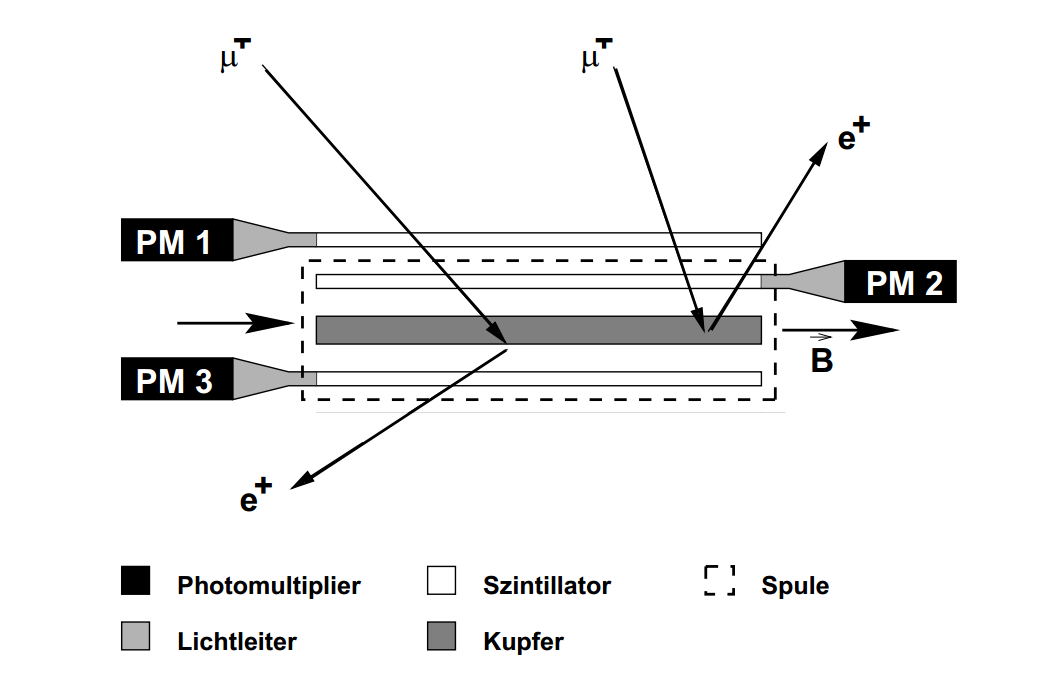
\includegraphics[width=.5\columnwidth]{./Versuchsaufbau.png}
	\caption{Schematische Abbildung der Messanordnung.}
	\label{fig:aufbau}
\end{figure}

\subsubsection{Szintillator}
\label{sec:szinti}

Wenn in das Szintillatormaterial, das organischer oder anorganischer Natur sein kann, ionisierende
Strahlung eintritt, wie in diesem Versuch hauptsächlich Myonenstrahlung sowie Strahlung aus 
Elektronen und Positronen, entstehen bei Stoßprozessen innerhalb des Materials Elektronen, Löcher
oder Elektron-Loch-Paare (so genannte Exzitonen). Diese diffundieren durch das Detektormaterial
bis sie auf einen Aktivator treffen, bei dem diese Ladungsträger rekombinieren und dadurch
Photonen emittieren. Diese Photonen haben nun eine Wellenlänge, die sich im Bereich sichtbaren
Lichts befindet, und gelangen durch den Szintillator zum angeschlossenen Photomultiplier.

\subsubsection{Photomultiplier}
\label{sec:photomulti}

Im Photomultiplier (PM) treffen die Photonen aus dem Szintillator zunächst auf eine Photodiode,
die die auftreffenden Photonen mit Hilfe des Photoeffekts in ein elektrisches Signal umwandelt.
Je nachdem wie viele Photonen auftreffen, kann dieses Signal aus nur wenigen Elektronen bestehen.
Um das Signal messen zu können, wird es in einem Sekundärelektronenvervielfältiger verstärkt.
In diesem Vervielfältiger liegt eine Hochspannung an, sodass sich alle Elektronen in eine Richtung
bewegen. Während ihrer Reise gen Anode treffen sie immer wieder auf Dynoden aus denen sie 
weitere Elektronen herauslösen. Dadurch wird die Zahl der Elektronen exponentiell größer.
Die Elektronenanzahl, die am Ende gemessen wird, hängt dabei erstens von der Anzahl der Photonen
ab, die eingangs auf die Photodiode getroffen sind, aber auch von der Hochspannung, weswegen diese
genau eingestellt werden muss.

\subsection{Likelihood-Methode}
\label{sec:likemeth}

Die so genannte Maximum-Likelihood-Methode ist eine Methode mit der man aus zuvor gemessenen Daten
eine gesuchte, aber natürlich unbekannte, Größe abschätzt. Man bestimmt also den Wert, für den
es am wahrscheinlichsten ist, die zuvor gemessenen Daten zu messen.\\

Um diese Methode anwenden zu können, muss die Wahrscheinlichkeitsdichteverteilung \(P(\vec{x},\tau)\)
der gemessenen Werte in Abhängigkeit der unbekannten, also gesuchten Größe
\(\tau\) bekannt sein (\(\vec{x}\) meint hier die Gesamtheit der Messdaten). 
Mit Hilfe dieser Verteilungen ergibt sich die Likelihood-Funktion \(L\) 
dann aus dem Produkt über all dieser.

\begin{equation}\label{eq:likefkt}
 L(\vec{x},\tau) = \prod_{i=1}^{N} P(x_i,\tau)
\end{equation}

Um nun aus~\ref{eq:likefkt} den wahrscheinlichsten Wert herauszufinden, muss diese Funktion
maximiert werden. Praktisch maximiert man allerdings den Logarithmus der Funktion, da dies
einfacher ist, weil sich das Produkt dadurch in eine Summe umwandelt. Es muss also gelten 
(\(\hat\tau\) meint hier den wahrscheinlichsten Wert):

\begin{equation}\label{eq:likediff}
 \frac{d \ln L}{d a} \mid_{\tau = \hat{\tau}} = 0
\end{equation}

In diesem Versuch gibt es drei verschiedene Möglichkeiten, die Maximum-Likelihood-Methode
anzuwenden, die im Folgenden kurz umrissen werden sollen.

\subsubsection{Max-Log-Likelihood-Methode und das exponentielle Zerfallsgesetz}
\label{eq:likezerfall}

Myonen zerfallen nach dem exponentiellen Zerfallsgesetz:

\begin{equation}\label{eq:zerfall}
 N(t) = N(t_0) \cdot \exp[-\frac{t-t_0}{\tau}]
\end{equation}

Die Wahrscheinlichkeitsdichte ergibt sich damit zu:

\begin{equation}\label{eq:wahrzerfall}
 P(t_i,\tau) = \frac{1}{\tau} \cdot e^{-t_i/\tau}
\end{equation}

Diese Gleichung gilt allerdings nur für eine unendliche Beobachtungszeit, da hier das Integral
von \(t = 0\) bis \(t = \infty\) 1 ergibt.
Da eine Beobachtungszeit solcher Länge unmöglich zu realisieren ist, muss~\ref{eq:wahrzerfall}
für Zeiten bis maximal \(T\) normiert werden:

\begin{equation}\label{eq:modzerfall}
 P(t_i,\tau) = \frac{1}{\tau}e^{-t_i/\tau} \cdot \frac{1}{1-e^{-\frac{T}{\tau}}}
\end{equation}

Daraus folgt:

\begin{equation}\label{key}
 \ln L = \sum (-\frac{t_i}{\tau} - \ln\tau - \ln(1-e^{-T/\tau}))
\end{equation}

und

\begin{equation}\label{key}
 \hat\tau = \frac{1}{N} \sum t_i + \frac{T e^{-\frac{T}{\tau}}}{1-e^{-\frac{T}{\tau}}}
\end{equation}

Bei dieser Methode muss in diesem Experiment allerdings beachtet werden, dass keine \(N\)
unterschiedliche Zeiten, sondern \(K\) Kanäle mit \(N_i\) Counts im \(i\)-ten Kanal gemessen
werden. Jeder Messwert ist mit einer statistischen Messungenauigkeit \(\sqrt{N_i}\) behaftet.
Unter Berücksichtigung dieser Besonderheiten folgt für \(\hat\tau\):

\begin{equation}\label{key}
 \hat\tau = \frac{1}{N} \sum_{k=1}^{K}N_k\cdot t_k + Korrektur
\end{equation}

Für die Standardabweichung ergibt sich aus der Fehlerfortpflanzung:

\begin{equation}\label{key}
 \sigma_{\hat\tau} = \frac{1}{N} \sqrt{\sum N_k \cdot t_k^2}
\end{equation}

\subsubsection{Max-Likelihood-Methode und die Poissonverteilung}
\label{sec:likepoisson}

Da es sich bei diesem Experiment um Zählmessungen handelt (man hat \(f_i\) Einträge pro
Zeitkanal \(i\)), ist die Poissonverteilung mit dem mittleren Erwartungswert \(f\) eine gute 
Möglichkeit, die Messungen statistisch zu  beschreiben. Die Wahrscheinlichkeit, \(N_i\) Einträge 
im \(i\)-ten Zeitkanal zu messen, wird durch folgende Wahrscheinlichkeitsdichteverteilung 
beschrieben:

\begin{equation}\label{eq:poisson}
 P(N_i,f_i) = \frac{f_i^{N_i} \cdot e^{-f_i}}{N_i !}
\end{equation}

Mit der Varianz um für \(N_i\) um den entsprechenden Mittelwert \(f_i\):

\begin{equation}\label{key}
 \sigma_i^2 = f_i
\end{equation}

Es ergibt sich für die logarithmierte Likelihood-Funktion:

\begin{equation}\label{key}
 -2\ln L = -2\sum_{i} N_i \ln f_i +2N +2\sum_{i} \ln(N_i!)
\end{equation} 

Da der Term \(2N +2\sum_{i} \ln(N_i!)\) nicht von der gesuchten Größe \(\tau\) abhängt, reicht es
aus \(-2\sum_{i} N_i \ln f_i\) über \(\tau\) aufzutragen.

\subsubsection{Max-Log-Likelihood-Methode und Gaußverteilung}
\label{sec:likegauss}

Für den Grenzfall großer Erwartungswerte, bedeutet mindestens \(f_i > 10\) pro Kanal, also für
eine große Observationszeit (hier eine Langzeitmessung, die eine Woche lang läuft), geht die 
Poissonverteilung in die Gaußverteilung über. Für das hier durchgeführte Experiment ergibt sich
die Wahrscheinlichkeitsdichteverteilung zu:

\begin{equation}\label{eq:wahrgauss}
 P(N_i,\tau) = \frac{1}{\sqrt{2\pi \sigma_i^2}} \cdot \exp[-\frac{(N_i-f_i)^2}{2\sigma_1^2}]
\end{equation}

Analog zur Poissonverteilung folgt für die logarithmierte Likelihoodfunktion:

\begin{equation}\label{key}
 -2\ln L = \sum_{i}\ln (2\pi\sigma_i^2) + \sum_{i} \frac{(N_i - f_i)^2}{\sigma_i^2}
\end{equation}

Da der erste Summenterm durch die Näherung \(\sigma_i(f_i) = \sqrt{f_i} \approx \sqrt{N_i}\) nicht
von \(\tau\) abhängt, kann dieser bei der Bestimmung von \(\hat{\tau}\) vernachlässigt und nur
der zweite Term betrachtet werden, der eine \(\chi^2\)-Verteilung beschreibt.

\begin{equation}\label{eq:chi}
 \chi^2 = \sum_{i} \frac{(N_i - f_i)^2}{\sigma_i^2}
\end{equation}

Die \(\chi^2\)-Funktion beschreibt wie stark eine gemessene Häufigkeit von der erwarteten abweicht.
Diese quadratische Abweichung wird durch die Varianz normiert, damit Werte mit einer hohen
Ungenauigkeit weniger stark in die Gesamtsumme einfließen. Idealerweise sollte der \(\chi^2\)-Wert
also möglichst klein werden, allerdings auch nicht zu klein, da sonst die Möglichkeit besteht, die
Ungenauigkeiten überschätzt zu haben.\\

Entsprechend wird bei dieser Methode der wahrscheinlichste oder beste Wert für \(\hat\tau\) durch
Minimierung der \(\chi^2\)-Funktion bestimmt.

\section{Durchführung und Auswertung}
\label{sec:ausw}

\subsection{Vorversuch}
\label{sec:vorversuch}

\subsubsection{Messung von Myon-Pulsen}
\label{sec:pulse}

Zuerst wurden die drei PM-Signale gemeinsam mit dem Koinzidenzsignal (123) für die ungestoppten
Myonen auf je einen Oszilloskopkanal. Die Spannungen der PMs wurden anschließend auf
\(U_{1,HV} = \SI{2300}{\volt}\), \(U_{2,HV} = \SI{2300}{\volt}\) und \(U_{3,HV} = \SI{2100}{\volt}\) eingestellt.

Das Oszilloskop wurde nun mit dem Koinzidenzsignal getriggert, damit es "weiß", wann es eine
Messung aufnehmen soll.
Danach wurde die Anzeige des Oszilloskops so eingestellt, dass die Peaks deutlich zu erkennen
waren, um die Höhe jedes der drei PM-Peaks zu messen. Dazu wurde mit Hilfe der Start-/Stopptaste
des Oszilloskops nach wenigen Sekunden das Bild eingefroren. Dabei wurde es vermieden auf den
Bildschirm zu sehen, um eine mögliche Beeinflussung und damit Verzerrung der Messergebnisse zu
verhindern. Mit Hilfe der ... wurde nun die Höhe von je 50 Peaks vermessen.

\section{Verzeichnisse}

\label{sec:literatur}

\listoffigures

\listoftables

\printbibliography
\end{document}
